% !TEX encoding = UTF-8 Unicode
\documentclass[11pt,a4paper]{report}		                                   

\usepackage{graphicx}
\usepackage{a4}
\usepackage[T1]{fontenc}
\usepackage[utf8]{inputenc}
\usepackage[ngerman]{babel}

\usepackage{wrapfig}  
\usepackage{acronym}
\usepackage{enumitem}
\usepackage[ampersand]{easylist}

\usepackage{listings}
\usepackage{color}
\usepackage{graphicx}
\usepackage{float}

\usepackage{caption}
\captionsetup{margin=8pt,font=footnotesize,format=hang}

\usepackage{url}

%Platzierung von Tabelle in Kapitel erzwingen 
\usepackage[section]{placeins}

%Tabellen
\usepackage{booktabs}
\usepackage[table,xcdraw]{xcolor}

\usepackage{chngcntr}
\counterwithout{figure}{chapter} %Kapitelübergreifende Bildnummerierung
\counterwithout{table}{chapter} %Kapitelübergreifende Tabellennummerierung

%Listings
\usepackage{listings} 
\lstset{
	  numbers=none,
	  numberstyle=\tiny,
	  numbersep=5pt,
	  captionpos=b,
	  showstringspaces=false,
	  basicstyle=\footnotesize\ttfamily,
	  numberbychapter=false
	  }
\lstset{language=Java}
\renewcommand{\lstlistingname}{Auflistung}
\renewcommand{\lstlistlistingname}{Auflistungen}
 
%Baumstruktur
\usepackage{tikz}
\usetikzlibrary{arrows,shapes,positioning,shadows,trees}

\tikzset{
	basic/.style = {draw, text width=2m, drop shadow, font=\sffamily, rectangle},
	root/.style = {basic, rounded corners=2pt, thin, align=center,
		fill=green!30},
	level 2/.style = {basic, rounded corners=6pt, thin,align=center, fill=green!60,
		text width=8em},
	level 3/.style = {basic, thin, align=left, fill=pink!60, text width=6.5em}
}

%Kapitelüberschriften
 \usepackage{fancyhdr} %Fancy Header
 \pagestyle{fancy}
 \fancyhead{}  
 \fancyhead[RE,RO]{\normalsize\sffamily \thechapter \ \leftmark} 
\cfoot{ \thepage}
 \renewcommand{\headrulewidth}{0pt}  
 \renewcommand{\chaptermark}[1]{\markboth{#1}{}}
 
 % set colors for links and URLs
 \usepackage[
 colorlinks=true,
 urlcolor=black,
 linkcolor=black,
 citecolor=black
 ]{hyperref}
 
%Fußnoten
\usepackage{scrextend} %Formatierung der Fuߟnoteneinträge
\deffootnote{1.5em}{1em}{ %Fußnoten Formatierung
	\makebox[1.5em][l]{\thefootnotemark}} % [l]-->Links

%handle subsections
\setcounter{secnumdepth}{3}
\setcounter{tocdepth}{3}

% Literatur - Achtung alphadin file angepasst!
\bibliographystyle{alphadin}




%Eigene Commands, falls gewuenscht
\newcommand{\umbruch}{\\ \noindent}		%Zeilenumbruch
\newcommand{\absatz}{\\ \\ \noindent}	%Absatz ohne einrücken
\newcommand{\extra}[1]{\emph{#1}} 		%Fremdworte, Englische Worte, ... kursiv

\renewcommand\lstlistingname{Quelltext} % Change language of section name

\newcommand{\thema}{Data Analytics}
\newcommand{\untertitel}{Einführung in ESPER}
\newcommand{\autoren}{Clemens Grabow (289116)\linebreak Lukas Groß (296836)}
\newcommand{\abgabedatum}{29.06.2018}
\newcommand{\arbeitsTyp}{Ausarbeitung}

\begin{document}

\include{front/cover}

\pagenumbering{gobble}
\tableofcontents
	\thispagestyle{empty}
\clearpage 
\pagenumbering{arabic}

% So werden Kapitel inkludiert
% \include{chapters/chapterName}
% !TEX encoding = UTF-8 Unicode
\chapter{Motivation}
In Zeiten der Digitalisierung und BigData, sind Informationen in Echtzeit immer wichtiger.
Riesige, stetig steigende Datenmengen fordern die IT heraus, um Lösungen zu finden.
 
Hinzu kommt die Fähigkeit agil auf die Informationen reagieren zu können, wozu Agile und Geschäfts-Prozesse benötigt werden. 
Durch rasch und stetig wandelnde Marktkonstellationen- und Bedingungen wird es immer wichtiger für Organisationen, sich schnell und individuell anpassen zu können. Um den Überblick zu behalten benötigt es eine einheitliche, lose gekoppelten Architektur, welche in Echtzeit große Datenmengen, im Optimalfall auch in einem verteilten System, verarbeiten kann. Dies stellt auch die Softwareentwicklung vor Herausforderungen.
Erforderlich sind Tools und Bibliotheken, mit welchen die Ereignisverarbeitung skalierbar in Echtzeit durchgeführt werden kann. Tools wie Esper stellen Lösungen dar, um diesen Problemen durch CEP mithilfe einer Event-Engine entgegenzuwirken. Hierdurch soll eine flexible Architektur und resultierend hieraus ein agiles Vorgehen ermöglicht werden.

Um den Studierenden an der HTWG zu ermöglichen, im Bereich Data Analytics, Fallstudien durchzuführen und Architekturen zu untersuchen, wird das Tool Esper, als Repräsentant der Event-verarbeitenden Lösungen, eingeführt.
Das Ziel ist die Grundlagen von Esper zu vermitteln. Dies führt den Leser von der Grundlagentheorie, über die Installation und erste Schritte hinweg, bis hin zum lauffähigen Beispiel.
Dabei richtet sich diese Arbeit an die Leser, welche eine eigene Lösung im Bereich Ereignisorientierung erstellen möchten.
Dem Leser soll einen Einblick in Esper ermöglicht werden, um danach in der Lage zu sein, die Lösung zu verstehen und technisch umsetzen zu können.
% !TEX encoding = UTF-8 Unicode
\chapter{Szenario}
\label{Szenario}
Um die Beispiele in dieser Ausarbeitung zu verdeutlichen, wird das Szenario ''Online Poker Portal'' verwendet. Der Fokus des Casinos liegt auf Gewinn-Maximierung im Bereich des Kartenspiels Texas Hold 'em.
\absatz
Hierzu ist es wichtig, dass alle Spiele aufgezeichnet werden und das der Event-Strom (Daten wie Spielzüge, Gewinnsumme und Siegesblatt) analysiert wird. 
Durch die Analyse ist es möglich, eine Betrugserkennung durchzuführen, so werden sehr unwahrscheinliche Glückssträhnen (z.B. Mehrmals mit Royal Flush gewinnen) betrachtet.
Betrugsversuche wie Kartenzählen kann nicht erkannt werden, dies ist eine Grenze des Systems. Jedoch ist es möglich zu erkennen, ob z.B. zu viele Karten eines Typs im Spiel sind.
Außerdem sollen Spieler, die Durchschnittlich zu viel gewinnen und eine gewisse Summe übersteigen, erkannt und aus dem Casino entfernt werden.
% !TEX encoding = UTF-8 Unicode
\chapter{Konzepte}
Die Konzepte welche Esper verwendet werdet, dienen dazu, den kompletten Ereignisfluss von der Aktion bis zur Verarbeitung und nachfolgenden Aktionen, abzubilden.
Ereignisse werden dezentral gefeuert und sind, durch die Registrierung der Ereignistypen auf dem Ereignis-Prozessor, klar definiert. Je nach hinterlegtem Regelwerk, werden diese, von einer Event-Engine, erfasst und verarbeitet oder ignoriert. Zur Regeldefinition dienen Muster, welche als Statements umgesetzt werden. Die Ereignismuster können verschiedene Techniken verwenden, nach denen der Ereignisstrom untersucht wird. 
Wie die Konfiguration, mit Ereignisdefinition-, Registrierung, sowie das Feuern und Verarbeiten der Ereignisse, in Esper umgesetzt wird, ist in Kapitel \ref{kapitel_architektur} beschrieben.
Nähere Informationen zu den Konzepten und weitere, hier nicht näher erläuterte, Möglichkeiten von Esper können der Dokumentation \cite{EsperRef2018} entnommen werden.
Im folgenden werden die Konzepte von Esper erläutert. Anschließend wird jeweils Bezug auf einen Casino-Anwendungsfall genommen und aufgezeigt.


\section{Statements}
\label{statements}
Statements dienen dazu Muster zu definieren, mit deren Hilfe die Event-Engine den Datenstrom analysiert. Hierzu existiert die \acf{EPL}, welche stark an den Syntax von SQL erinnert. Mit ihr werden die Ereignismuster definiert und die Ereignisverarbeitung umgesetzt.
\cite{EsperRef2018}[7-8]

\section{Select}

Quelltext \ref{basic_select} zeigt ein einfaches Select-Statement. Resultierend hieraus, wird der \acf{EP} auf alle Ereignisse vom Typ \texttt{Action} reagieren und diese bei Eintritt erfassen. 
\begin{lstlisting}[caption={Statement einfache Selektion}\label{basic_select},captionpos=b,language=SQL]

select * from GameActionEvent

\end{lstlisting}
Der Ablauf wird beispielhaft in Abbildung \ref{basic_select_img} grafisch dargestellt. Sie werden unverändert weitergegeben. Dieses Statement wird im dem Casino eingesetzt, um über sämtliche Züge informiert zu werden. Erkennbar ist jedoch nicht, welcher Zug zu welchem Spiel, etc. gehört. Um Ereignisse feingranular untersuchen zu können, werden weitere Techniken benötigt, welche beispielsweise nach Attributen filtern können.
\cite{EsperRef2018}[8-9]

\begin{figure}[h]
	\centering
	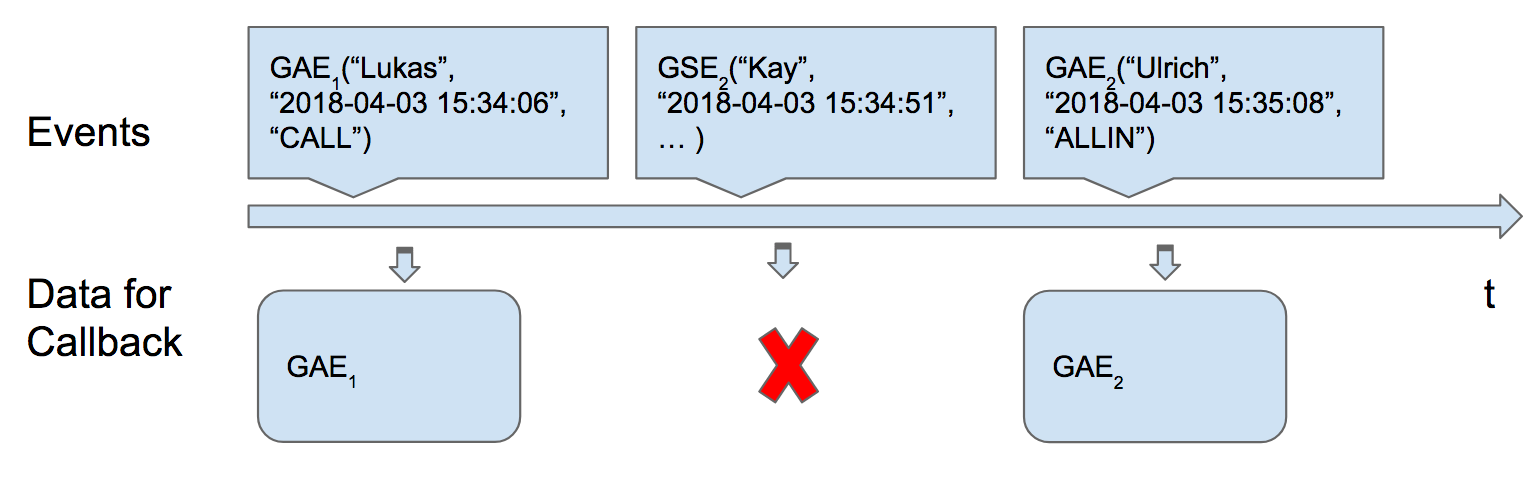
\includegraphics[width=\textwidth,height=\textheight, keepaspectratio]{images/statement_basic_select.png}
	\caption{Ablauf einfache Selektion}
	\label{basic_select_img}
\end{figure}

\section{Filter}

Die Filterfunktion ist eine geeignete Möglichkeit, die Selektion aus dem Ereignisfluss auf bestimmte Attribut-Werte zu beschränken. Wie das Beispiel in Quelltext \ref{filter_select} veranschaulicht, können, wie im SQL Syntax, Ereigniseigenschaften beschränkt werden.
\begin{lstlisting}[caption={Statement mit Filter}\label{filter_select},captionpos=b,language=SQL]

select playerName, deck from GameEndEvent(deck="ROYAL_FLUSH")

\end{lstlisting}
Wie Quellcode (\ref{filter_select}) zeigt, selektiert die Event-Engine die Attribute \texttt{playerName} und \texttt{deck} der auftretenden Ereignisse vom Typ \texttt{GameEndEvent}. Anschließend wird mit \texttt{GameEndEvent(deck="ROYAL\_FLUSH")} überprüft, ob der Wert des Deck-Attributes im Endevent, einem Royal-Flush entspricht.
Der Ablauf des Quellcodes wird in Abbildung \ref{filter_select_img} grafisch aufgezeigt. Gut zu sehen, ist, dass nur die End-Events erfasst werden, welche dem Attribut-Wert entsprechen. Weil nur ein Spieler mit einem Royal-Flush-Blatt gewinnt, wird auch nur dieses Ereignis verarbeitet.
Das Casino benötigt ein solches Statement, um zu erfahren, wer welches Spiel mit welcher Hand gewonnen wird. Um jedoch, einen Spieler mit oftmaligem Glück zu entdecken, ist die Anzahl der Siege erwünscht. Hierfür können die selektierten Daten, mit weiteren Funktionen aggregiert werden.
\cite{EsperRef2018}[10-11]
\begin{figure}[ht]
	\centering
	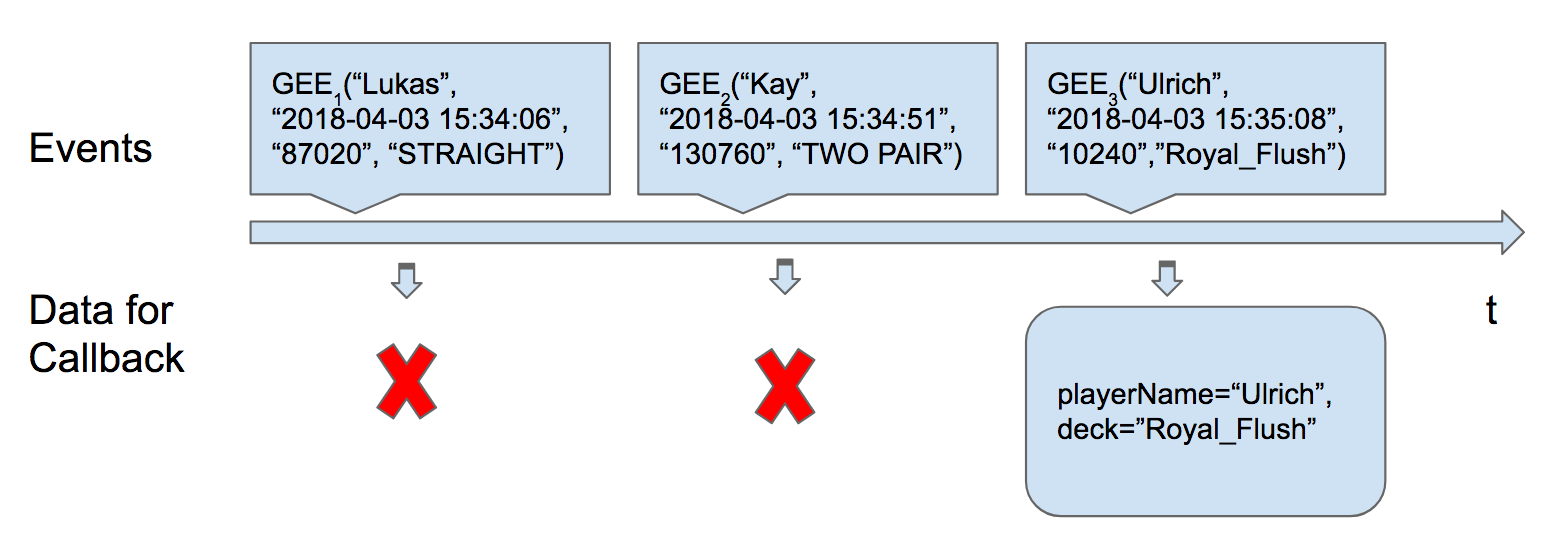
\includegraphics[width=\textwidth,height=\textheight, keepaspectratio]{images/statement_basic_filter.png}
	\caption{Ablauf gefilterte Selektion}
	\label{filter_select_img}
\end{figure}

\section{Aggregation}

Um zu erfahren, welcher Spieler wie oft gewonnen hat wird die Aggregationsfunktion \texttt{count(playerName)} verwendet.
\begin{lstlisting}[caption={Statement mit Aggregation}\label{aggregation_select},captionpos=b,language=SQL]

select playerName, count(playerName) as wins, deck from GameEndEvent

\end{lstlisting}
'' gespeichert.
Der Ablauf hierbei ist in Abbildung \ref{aggregation_select_img} veranschaulicht. 
Zudem sind weitere Aggregationsfunktionen wie \texttt{sum()} oder \texttt{avg()} in Esper verfügbar.
Im Casino fällt auf, dass sich die Spielenden der Vortage in den zu analysierenden Daten befinden. Um nur die Daten des aktuellen Tages auswerten zu können, sind Beschränkungen des auszuwertenden Ereignisstroms erforderlich. Die \acf{EPL} bietet hierfür sogenannte Data-Windows.
\cite{EsperRef2018}[9-10]

\begin{figure}[ht]
	\centering
	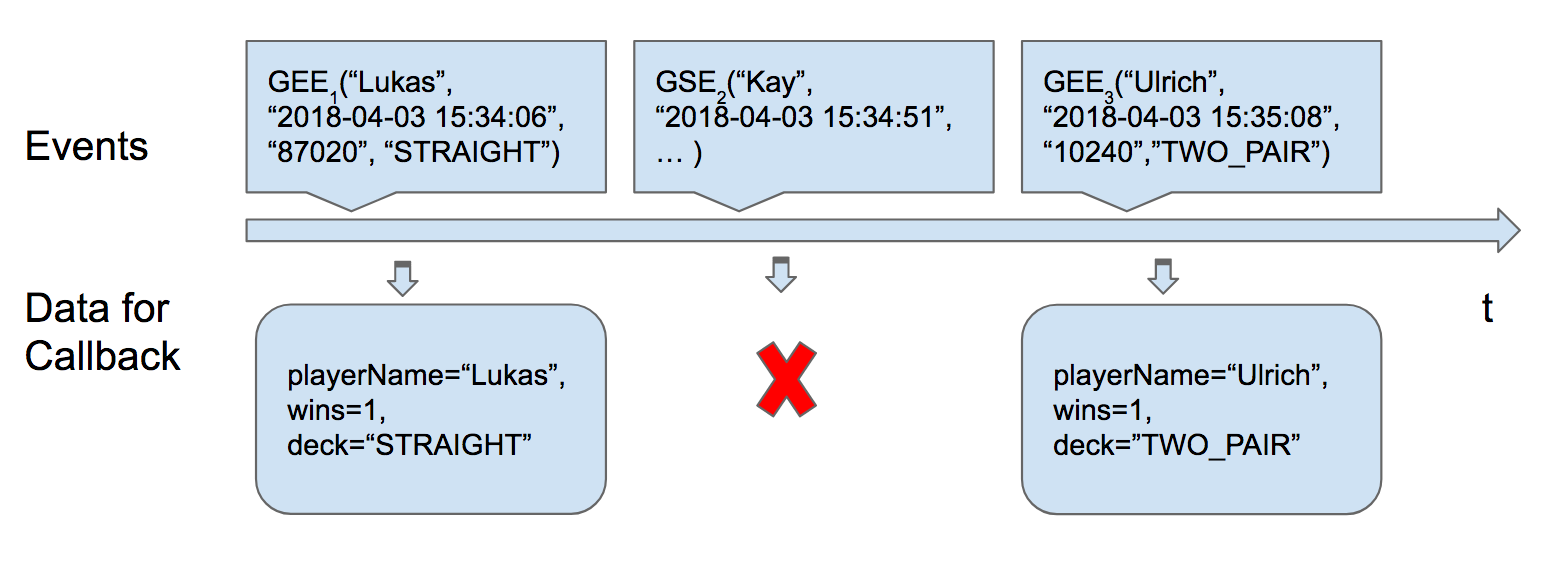
\includegraphics[width=\textwidth,height=\textheight, keepaspectratio]{images/statement_basic_aggregation.png}
	\caption{Ablauf Selektion mit Aggregation}
	\label{aggregation_select_img}
\end{figure}

\section{Data-Windows}
\label{Data-Windows}
\begin{figure}[ht]
	\centering
	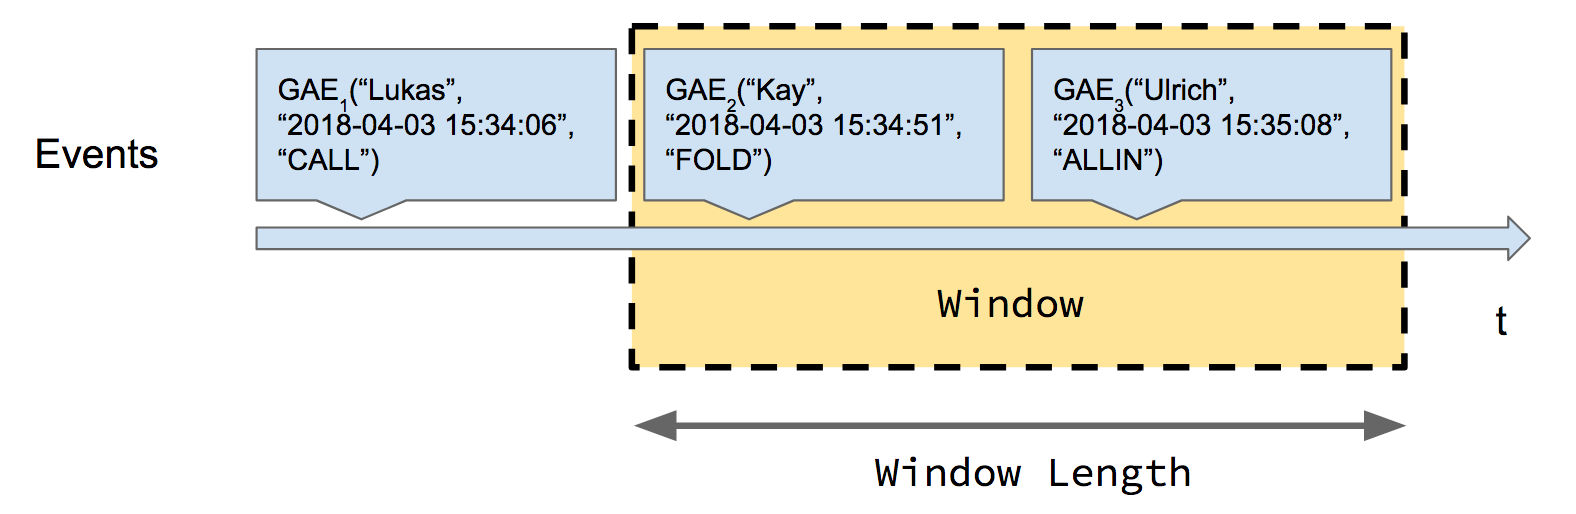
\includegraphics[width=\textwidth,height=\textheight,keepaspectratio]{images/data_window_length.png}
	\caption{Length Window}
	\label{LengthWindow}
\end{figure}

Mit dem \textbf{Length Window} können mehrere Events im Bezug zueinander betrachtet werden (Kausalität). Hierzu wird eine Länge angegeben (in der Abbildung wird die Länge 2 verwendet), welche angibt, wie viele Events zusätzlich zum aktuellen betrachtet werden sollen. In diesem Fall würde das aktuelle Event und das vorherige Event betrachtet werden. Die Art des Events wird im Statement angegeben. Für das obige Beispiel könnte dies folgendermaßen aussehen:

\begin{lstlisting}[caption={Statement mit Length Window}\label{length_select},captionpos=b,language=SQL]

select * from GameActionEvent.win:length(2)

\end{lstlisting}

\begin{figure}[ht]
	\centering
	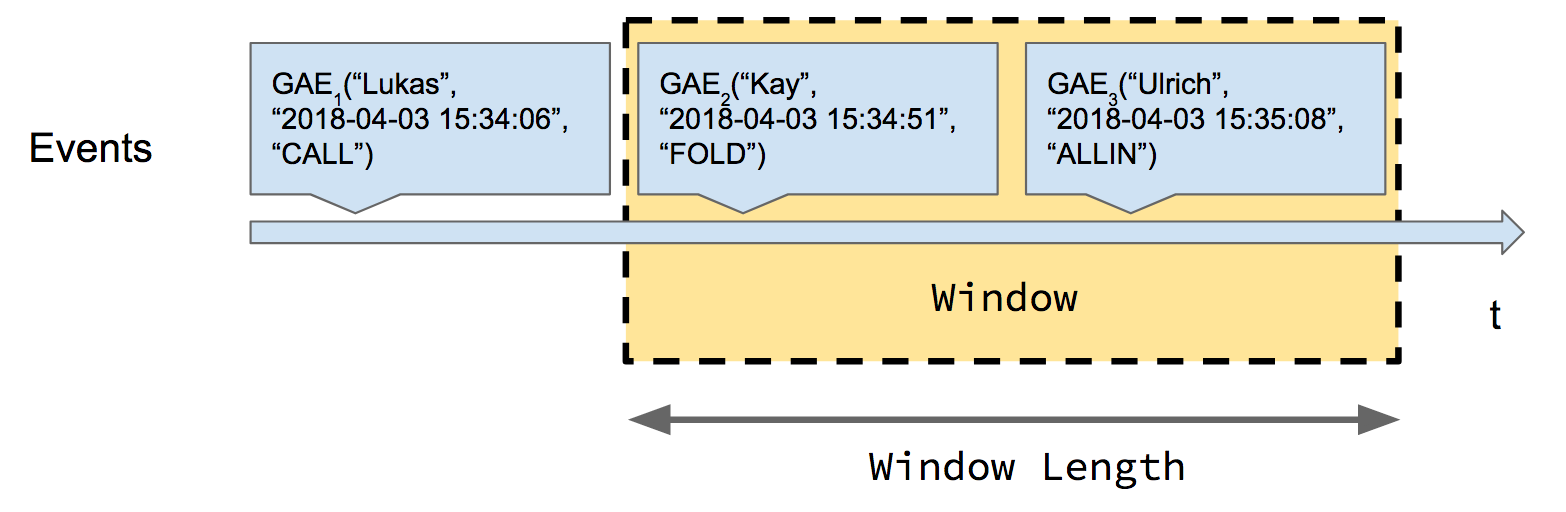
\includegraphics[width=\textwidth,height=\textheight,keepaspectratio]{images/data_window_length_batch.png}
	\caption{Length-Batch Window}
	\label{LengthBatchWindow}
\end{figure}

\begin{figure}[ht]
	\centering
	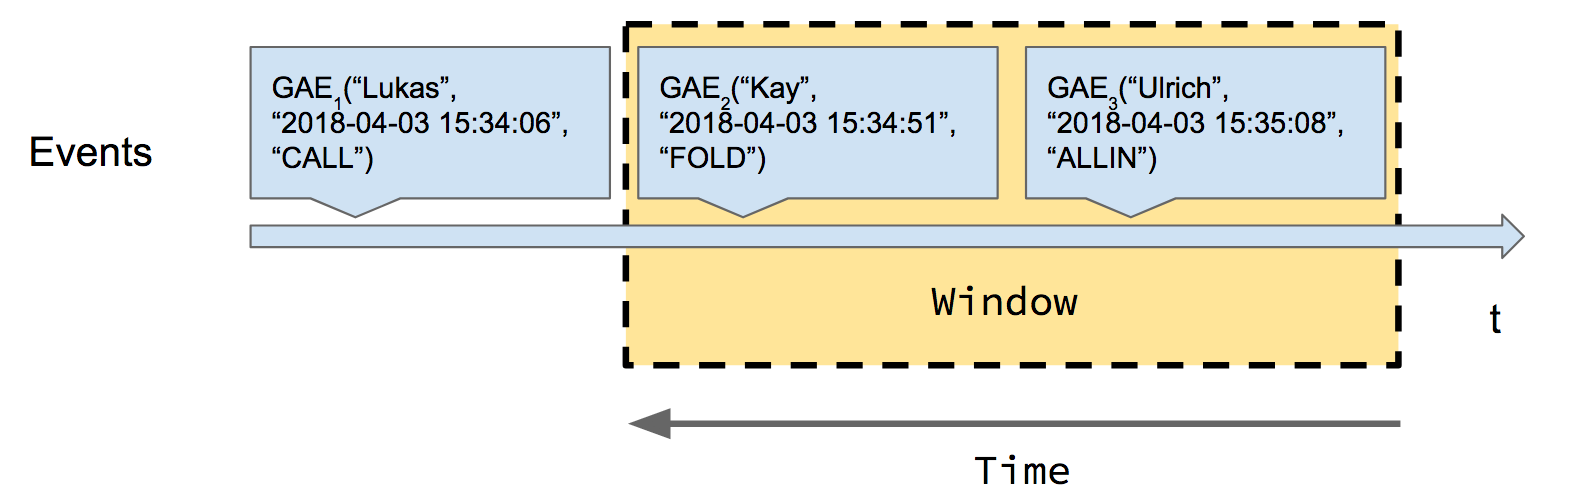
\includegraphics[width=\textwidth,height=\textheight,keepaspectratio]{images/data_window_time.png}
	\caption{Time Window}
	\label{TimeWindow}
\end{figure}

\begin{figure}[ht]
	\centering
	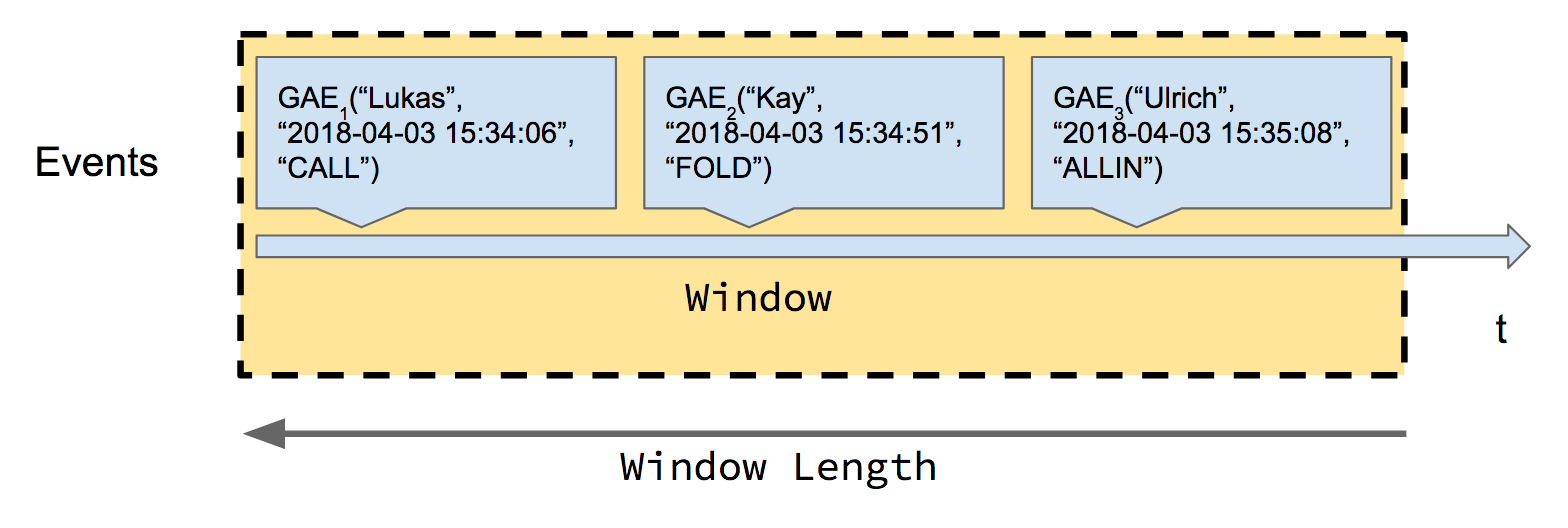
\includegraphics[width=\textwidth,height=\textheight,keepaspectratio]{images/data_window_keep_all.png}
	\caption{Keep-All Window}
	\label{KeepAllWindow}
\end{figure}

\section{Patterns}

Eine Alternative zu den Select-Satements stellen Abfragen nach Strukturen, sogenannte Patterns dar. Events, welche den Bedingungen entsprechen werden erfasst. Hierbei kommen verschiedene Elemente bei der Pattern-Definition zum Einsatz.
\cite{EsperRef2018}[25]

\begin{enumerate}
	\item \textbf{Kontrolloperator:} \texttt{every} definiert die Erstellung eines Pattern und regelt die Abarbeitung. Es wird alle(engl. every) auf das Ereignismuster zutreffende Ereignisse erfasst. Ein simples Pattern, welches alle Ereignisse vom Typ \texttt{GameActionEvent} erfasst, kann Quellcode \ref{basic_pattern} entnommen werden.
	Mit der \texttt{where}-Klausel können wie bei der Selektion weitere Bedingungen, definiert werden.
	
	\begin{lstlisting}[caption={Einfaches Pattern mit Where-Klausel}\label{basic_pattern}, captionpos=b,language=SQL]
	
	every GameActionEvent
	
	\end{lstlisting}
	
	\item \textbf{Logische Operatoren:} 
	Das Pattern kann, wie in Quellcode \ref{logic_pattern} veranschaulicht, durch logische Operatoren wie \texttt{and, or , not} zusammengesetzt werden. So kann wie in Quellcode \ref{logic_pattern} das Ereignismuster mit Bedingungen bestückt werden. In diesem Beispiel würden Events vom Typ \texttt{GameEnd} oder vom Typ \texttt{GameAction} erfasst werden.
	
	\begin{lstlisting}[caption={Pattern mit logischen Operatoren}\label{logic_pattern},captionpos=b,language=SQL]
	
	every a=GameActionEvent or b=GameActionEvent
	
	\end{lstlisting}
	
	\item \textbf{Nachfolge-Operator:}
	Der Nachfolge-Operator \texttt{->} tritt ein wenn das davor, gefolgt vom danach definierten Ereignis eintrifft. In Quellcode \ref{follow_pattern}  werden alle Endevents betrachtet, welche auf ein Aktionsevent folgen. Die Bedingung trifft zu, wenn der vorangegangene Zug ein Spielausstieg(\texttt{action = "FOLD"}) war.
	Wie im Quellcode zu erkennen ist, werden die Ereignisse in Variablen \texttt{a, b} gespeichert(bspw. \texttt{a=GameAction}). So können die Werte im nächsten Schritt weiterverwendet werden. Im Beispiel wird das Folgeevent (\texttt{b=GameEnd(a.playerName != b.playerName)}) überprüfen ob der Spieler-Name ungleich dem vorherigen ist und im Erfolgsfall erfasst. Auf diese Art lassen sich komplexe bedingte Ereignismuster definieren.
	
	\begin{lstlisting}[caption={Pattern mit Follow-Operator }\label{follow_pattern},captionpos=b,language=SQL]
	
	every a = GameActionEvent(action="FOLD") -> b =
	 GameEndEvent(a.playerName != b.playerName)
	
	\end{lstlisting}
	
	\item \textbf{Bedingungen:}
	Um Grenzen zu definieren, nach welcher das Pattern geprüft wird, dient die \texttt{where}-Klausel. Nach ihr können verschiedene Bedingungen, durch Konstellationen der Operatoren, angegeben werden.
	Meisten werden Vergleichsoperatoren wie \texttt{=, < , > , >=, <=, !=, <>, is null, is not null} und logische Kombinationen wie\texttt{and, or} verwendet. So können Ereignisse in Korrelation gestellt und ausgewertet werden. Die \texttt{where}- Klausel kann auch bei der Selektion verwendet werden.
	
	\item \textbf{Überwacher} (engl. Observer):
	Um Ereignisströme zu überwachen werden Observer verwendet, welche beispielsweise in einem Zeitintervall oder zu einem Zeitpunkt agieren. Sie können nach der \texttt{where}-Klausel angegeben werden. Beispielsweise kann ein Timer mit Intervall, durch \texttt{timer:interval} definiert werden. Ein Zeitpunkt wird
	mit \texttt{timer:at} festgelegt, eine Zeitspanne mit \texttt{timer:within}. Für das Casino wird der Überwacher auf ein Zeitintervall eines Werktages gesetzt, um nur die Ereignisse des aktuellen Tages zu erhalten. So fließen die historischen Daten nicht verfälschend in die Auswertung mit ein.
	
	\begin{lstlisting}[caption={Pattern mit Observer }\label{observer_pattern},captionpos=b,language=SQL]
	
	every a = GameActionEvent(action="FOLD") -> b =
	GameEndEvent(a.playerName != b.playerName)
	where timer:within(28800 seconds)
	
	\end{lstlisting}
	
\end{enumerate}


\section{Partitions}

Esper bietet die Möglichkeit Abfragen zu partitionieren.
Hierzu wird ein zeitlicher Context mit \texttt{create context} erstellt.
\texttt{start} definiert den Start-, \texttt{end} den Endzeitpunkt.
Mit \texttt{after 28800 sec} wir die Dauer dynamisch auf eine Zeitspanne von acht Stunden gesetzt. Verwendet wird der erzeugte Context mit texttt{context OneWorkDay}. Diese Deklaration sorgt dafür, dass sich das darauffolgende \texttt{select}-Statement auf die Partition bezieht.
In Quellcode \ref{partitioned_pattern} wird mit dem ersten Statement eine achtstündige Partition erstellt. Diese wird in der zweiten Zeile verwendet, um die Spieler- und Spielzugnamen aller Aktionen eines Arbeitstagen zu erfassen.
\cite{EsperRef2018}[18]

\begin{lstlisting}[caption={Partitioniertes Pattern}\label{partitioned_pattern},captionpos=b,language=SQL]

create context OneWorkDay start @now end after 28800 sec

context OneWorkDay select playerName, action from GameActionEvent

\end{lstlisting}

\section{Kombinierte Statements}


% !TEX encoding = UTF-8 Unicode
\chapter{Umsetzung}
In diesem Kapitel wird beschrieben, wie Esper installiert werden kann. Anschließend wird die für die Ausarbeitung entwickelte Java-Anwendung gezeigt. Diese verwendet Esper im Kontext des Szenarios (siehe Kapitel \ref{Szenario}).

\section{Installation}
Für die Installation von Esper wird in dieser Ausarbeitung des Build-Tool \textbf{Apache Maven} verwendet. 
Dieses ermöglicht das automatisierte Herunterladen der Esper-Engine. Hierzu wird eine Konfigurationsdatei für Maven benötigt, die sogenannte \textbf{pom.xml}. Nachfolgend wird diese für das Szenario dargestellt:

\begin{lstlisting}[caption={Maven-Konfiguration}\label{lst:mavenKonfiguration},captionpos=t,language=XML]

<?xml version="1.0" encoding="UTF-8"?>
    <project xmlns="http://maven.apache.org/POM/4.0.0"
     xmlns:xsi="http://www.w3.org/2001/XMLSchema-instance"
     xsi:schemaLocation="http://maven.apache.org/POM/4.0.0
     http://maven.apache.org/xsd/maven-4.0.0.xsd">
		
     <modelVersion>4.0.0</modelVersion>

     <groupId>de.htwg.da</groupId>
     <artifactId>esper-sample</artifactId>
     <version>1.0-SNAPSHOT</version>

     <dependencies>
         <dependency>
             <groupId>com.espertech</groupId>
             <artifactId>esper</artifactId>
             <version>7.1.0</version>
         </dependency>
     </dependencies>
</project>
\end{lstlisting}

Wichtig ist hierbei das XML-Element \textbf{<dependencies>} welche die Abhängigkeiten enthält. Diese werden automatisch heruntergeladen, sobald Maven ausgeführt wird. In der Beispiel-Konfiguration gibt es nur eine Abhängigkeit, die für Esper.

Nach dem Download kann die Esper-Engine direkt bei der Entwicklung einer Java-Anwendung verwendet werden. Für andere Sprachen, sind unter Umständen Build-Tools zu verwenden, welche hier nicht beschrieben werden.

\section{Implementierung}
Dieses Kapitel beinhaltet die einzelnen Schritte der Implementierung des Szenarios (beschrieben in Kapitel \ref{Szenario}). Zu beginn werden die erzeugten Event-Klassen beschrieben, anschließend wird das Versenden der Events und deren Verarbeitung behandelt.

\subsection{Event-Klassen}

\begin{figure}[ht]
	\centering
	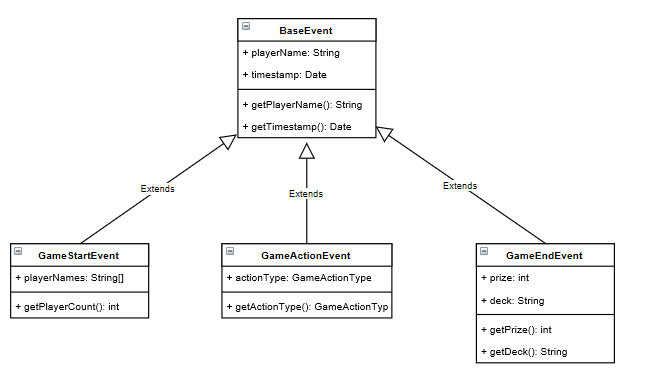
\includegraphics[width=\textwidth,height=\textheight,keepaspectratio]{images/Events.png}
	\caption{Event Klassen des Szenarios}
	\label{EventKlassen}
\end{figure}

Um das Szenario abzubilden werden verschiedene Event-Klassen benötigt. Mit diesem Begriff sind Klassen gemeint, die ein Event darstellen.
Als gemeinsame Basis dient die Event-Klasse \textbf{BaseEvent} (Siehe Abbildung \ref{EventKlassen}). Dieses Event beinhaltet den Spieler-Namen und einen Zeitstempel. Diese beiden Felder werden in allen Events benötigt.

Die Event-Klassen \textbf{GameStartEvent} und \textbf{GameEndEvent} bilden den Start und das Ende einer Poker-Partie ab. Zu Beginn (\textbf{GameStartEvent}) werden alle Spiel-Teilnehmer benötigt, gegen Ende (\textbf{GameEndEvent}) das Preisgeld und Kartendeck, welches gewonnen hat. Da beide Events von \textbf{BaseEvent} erben, besitzen sie automatisch einen Zeitstempel und den zugeordneten Spieler. Beim Spielstart wird der Name des ersten Spielers verwendet.

Im Laufe der Partie werden verschiedene Aktionen der Spieler durchgeführt. Diese sind durch die Event-Klasse \textbf{GameActionEvent} abgebildet. Das Event beinhaltet ein Feld für die Aktionsart (z.B. "rise", wenn ein Spieler erhöht hat).

\subsection{Architektur}
\label{kapitel_architektur}
Die nachfolgende Abbildung zeigt die Architektur von Esper. Dabei ist sie, auf die in der Umsetzung benötigten Komponenten, beschränkt.

\begin{figure}[ht]
	\centering
	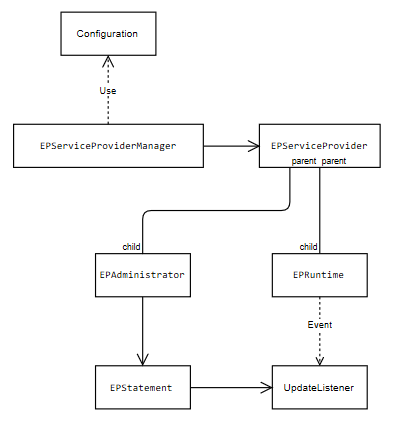
\includegraphics{images/Architektur.png}
	\caption{Architektur von Esper}
	\label{architektur}
\end{figure}

Die \textbf{Configuration}-Klasse wird verwendet, um die Esper-Engine zu konfigurieren. Unter anderem lassen sich dort die Event-Typen registrieren, die verarbeitet werden sollen. Neben den Event-Typen, gibt es die Möglichkeit Plugins zu registrieren. 

Durch Plugins werden benutzerdefinierte Funktionen eingebunden (z.B für den Vergleich von Geo-Koordinaten).
Nachfolgend zeigt die Basis-Konfiguration der Umsetzung:

\begin{lstlisting}[caption={Basis-Konfiguration}\label{lst:basisKonfiguration},captionpos=t,language=JAVA]

import com.espertech.esper.client.Configuration
import de.htwg.da.esper.sample.event.GameActionEvent;
import de.htwg.da.esper.sample.event.GameEndEvent;
import de.htwg.da.esper.sample.event.GameStartEvent;

Configuration config = new Configuration();

// Register event types to observe
config.addEventType("GameStart",GameStartEvent.class.getName());
config.addEventType("Action", GameActionEvent.class.getName());
config.addEventType("GameEnd", GameEndEvent.class.getName());
\end{lstlisting}

In der Konfiguration werden die Event-Typen \textbf{GameStartEvent}, \textbf{GameActionEvent} und \textbf{GameEndEvent} registriert. Plugins werden nicht verwendet.

Über die \textbf{EPServiceProviderManager}-Klasse kann der \textbf{EPServiceProvider} erhalten werden:

\begin{lstlisting}[caption={EPServiceProvider}\label{lst:epServiceProvider},captionpos=t,language=JAVA]

import com.espertech.esper.client.*;

EPServiceProvider cep = EPServiceProviderManager.
getProvider("MyEsperProvider", config);
\end{lstlisting}


Der erste Parameter stellt eine eindeutige Bezeichnung für den Provider dar. Dadurch ist es möglich, mehrere \textbf{EPServiceProvider} und damit mehr als eine Esper-Engine parallel zu verwenden. Als zweiter Parameter wird die zuvor  erstellte Konfiguration (siehe Quelltext \ref{lst:basisKonfiguration}) verwendet.

Der \textbf{EPServiceProvider} hält die Referenzen auf die Klassen \textbf{EPAdministrator} und \textbf{EPRuntime}. 

\subsection{Events versenden}
Für das Versenden eines Events wird die Methode \textbf{sendEvent(...)} der Klasse \textbf{EPRuntime} verwendet (siehe Abbildung \ref{architektur}). Als Parameter kann eine beliebige Event-Klasse übergeben werden, wie nachfolgend mit einem \textbf{GameStartEvent} dargestellt:

\begin{lstlisting}[caption={Event versenden}\label{lst:fireEvent},captionpos=t,language=Java]

EPServiceProvider cep = EPServiceProviderManager.
			getProvider("MyEsperProvider",esperConfig);

final EPRuntime cepRT = cep.getEPRuntime();

// Fire sample event
cepRT.sendEvent(new GameStartEvent());
\end{lstlisting}

\subsection{Events generieren}
Damit die Events für das Szenario einfach erzeugt und versendet werden können, wird eine Hilfs-Klasse (\textbf{EventGenerator}) verwendet. Dieser ist zuständig für die Generierung von Beispiel-Events (z.B. \textbf{GameActionEvent}).

\begin{lstlisting}[caption={Event Generator}\label{eventGenerator},captionpos=t,language=Java]
public final class EventGenerator {
  private static String[] PLAYER_NAMES = {"Clemens", "Lukas", "Kathrin"};
  private static Random GENERATOR = new Random();
  
  public static GameActionEvent randomGameActionEvent() {
    final String playerName = randomPlayerName();
    final Date timestamp = randomTimestamp();
    final GameActionType gameActionType = randomGameActionType();
    return new GameActionEvent(playerName, timestamp, gameActionType);
  }

  private static GameActionType randomGameActionType() {
    int gameActionTypeIndex = GENERATOR.nextInt(GameActionType.values().length);
    return GameActionType.values()[gameActionTypeIndex];
  }

  private static String randomPlayerName() {
    int playerIndex = GENERATOR.nextInt(PLAYER_NAMES.length);
    String playerName = PLAYER_NAMES[playerIndex];
    return playerName;
  }

  private static Date randomTimestamp() {
    long timeStamp = System.currentTimeMillis();
    return new Date(timeStamp);
  }
}
\end{lstlisting}

Zur besseren Übersichtlichkeit sind nicht alle Methoden im Quellcode \ref{eventGenerator} enthalten.
Gezeigt wird, dass über den Aufruf der Methode \textbf{randomGameActionEvent()} ein zufälliges \textbf{GameActionEvent} erzeugt wird. Hierzu werden für das zu erzeugende Event ein zufälliger Spieler-Name, Zeitstempel und Aktionstyp generiert. Die möglichen Werte können konfiguriert werden. Im obigen Beispiel sind dies ''Clemens'', ''Lukas'' und ''Kathrin'' als Spieler-Namen, die aktuelle Zeit als Zeitstempel und ein zufälliger Aktionstyp aus den möglichen Aktionen in Poker.

\subsection{Events verarbeiten}
Für das Verarbeiten von Events wird ein Statement (siehe Kapitel \ref{statements}) benötigt, um die gewünschten auszuwählen und ein UpdateListener, um es anschließend zu verarbeiten. Dieser spezielle Listener ist in der Esper-Bibliothek enthalten und enthält nur eine einzige Methode. Nachfolgend zeigt eine beispielhafte Implementierung für das Szenario der Ausarbeitung:

\begin{lstlisting}[caption={UpdateListener}\label{updateListener},captionpos=t,language=Java]
public class GameActionListener implements UpdateListener {

public void update(EventBean[] newData, EventBean[] oldData) {
Object event = newData[0].getUnderlying();

System.out.println("------> Game action: " + event);
}
}
\end{lstlisting}

Der \textbf{UpdateListener}, in der Abbildung GameActionListener genannt, erhält in der Methode \textbf{update(EventBean[] newData, EventBean[] oldData)} die aktuellen Events als ersten und die vorherigen als zweiten Parameter. Dadurch ist es möglich auf Beziehung zwischen Events zu schließen (Kausalität).

Anschließend wird über eine \textbf{System out}-Anweisung die aktuelle Aktion ausgegeben. Sind mehr als 1 Event im ersten Parameter der Methode enthalten, wird nur das erste ausgewertet (Das neuste Element). Die anderen Elemente wurden bereits zuvor abgearbeitet, da der \textbf{UpdateListener}, in diesem Beispiel, auf ein Statement hört, welches ein Length-Window (siehe \ref{LengthWindow}) verwendet, dies ist in der Abbildung nicht dargestellt.

Dies bedeutet auch, dass sich die Logik innerhalb des \textbf{UpdateListener} immer auch auf das gegebene Statement beziehen sollte. Wird z.B. ein Length-Batch-window (siehe \ref{LengthBatchWindow}) verwendet, müssen alle Events verarbeitet werden, wenn der \textbf{UpdateListener} aufgerufen wird, da dies erst geschieht, wenn das Window genau so viele Events wie angegeben enthält. Bei einem Length-Window (siehe \ref{LengthWindow}) muss immer nur das Neuste verarbeitet werden, weil dort der \textbf{UpdateListener} bei jedem Event ausgelöst wird. 

Dies zeigt auch, wie Komplex in Esper die Steuerung der Weiterverarbeitung von Events werden kann. 
% !TEX encoding = UTF-8 Unicode
\chapter{Fazit}
Mit Esper lassen sich auch komplexe Event-Ströme Analysieren und Auswerten. Durch den In-Memory Ansatz, kann dies sehr effizient mit geringen Latenzen realisiert werden,
da Daten nicht auf der Festplatte bzw. in einer Datenbank gespeichert und wieder ausgelesen werden müssen.

Konzepte wie Data-Windows (siehe \ref{Data-Windows}) erlauben es, eine Kausalität zwischen Events herzustellen.
Damit ist gemeint, dass nicht nur das aktuelle Event betrachtet, sondern auch die Events, welche zum aktuellen Event geführt haben.

In der Umsetzung (siehe \ref{EventsVerarbeiten}) wird aber auch gezeigt, wie komplex die Weiterverarbeitung der Events werden kann. Die eingesetzten Statements und Konzepte wie Data-Windows (siehe \ref{Data-Windows}) spielen dort eine große Rolle.

Ziel dieser Ausarbeitung war es, eine Einführung in Esper zu geben und die Grundlegenden Konzepte zu erläutern. Dieses Ziel wurde nach Meinung der Autoren erreicht, in der Arbeit werden die grundlegenden Konzepte von Esper erläutert und eine Anleitung für den Einsatz von Esper wird beschrieben.


\bibliography{bib/literatur_esper}
\addcontentsline{toc}{chapter}{Literaturverzeichnis}

% !TEX encoding = UTF-8 Unicode
\chapter*{Abkürzungsverzeichnis}
\addcontentsline{toc}{chapter}{Abkürzungsverzeichnis}

\begin{acronym}[Bash]
	\acro{CEP}{Complex Event Processing}
\end{acronym}

\end{document}